  % ---------------------------------------------------------------------------
  \section{Synthetic Ground-Truth Validation}
  \label{app:synthetic}
  % ---------------------------------------------------------------------------

  To test whether the certificates recover known hidden influence, we construct
  a synthetic agent whose hidden-state entropy and decision relevance are
  controlled by design. A binary hidden variable $H \sim \text{Bern}(0.5)$
  injects influence of strength $\beta_h$ into the action logits; the
  unlogged-channel capacity $c_H = H(H) = 1$ bit is known. Since $H$ is also a
  deterministic hidden-state witness, the non-recoverability lower certificate
  satisfies $\varepsilon_\text{unrec}^\text{LB}=H(H\mid\tilde T_t)=1$ bit. We
  run the structural min-cut budget
  ($\varepsilon_\text{state}^\text{UB}=1$ bit), the witness certificate, and the
  proxy CE-diff estimator on $1{,}000$ trajectories at five influence levels.

\begin{figure}[ht]
\centering
\small
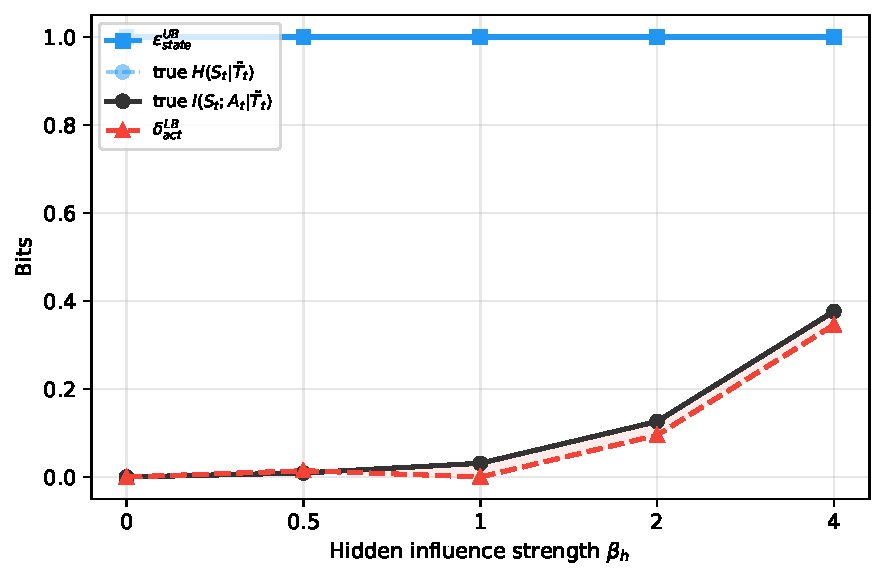
\includegraphics[width=0.55\textwidth]{figures/synthetic_gt.pdf}
\caption{Synthetic calibration: state and witness certificates equal the true
1-bit value, while $\delta_\text{act}^\text{LB}$ tracks conditional MI. Low-$\beta_h$
negatives reflect estimator variance near the noise floor.}
\label{fig:synthetic}
\end{figure}

  Fig.~\ref{fig:synthetic} shows
  $\varepsilon_\text{unrec}^\text{LB}
  =\varepsilon_\text{state}^\text{UB}=1$ bit, matching the true hidden entropy
  because the hidden variable is both the only unlogged channel and a measured
  witness. The dynamic lower bound $\delta_\text{act}^\text{LB}$
  tracks the true conditional MI from below at all tested influence levels
  ($\beta_h \geq 1$); negative CE-diff values at $\beta_h=0$ reflect
  finite-sample variance around a near-zero true MI.

  The Qwen deployment has a near-deterministic baseline that suppresses the
  proxy signal ($H(A_t \mid \tilde T_t) \approx 0$). The synthetic environment
  instead injects controlled stochasticity ($H = 1$ bit of hidden-state
  entropy). Without that observational bottleneck, the proxy certificate
  $\delta_\text{act}^\text{LB}$ tracks the true conditional-MI curve from below
  in the tested range. The validation shows that the proxy certificate can
  become tight when structural capacity is behaviorally active \emph{and} the
  observational ceiling permits detection.
